\documentclass[10pt]{proc}

\usepackage{amsmath}    % need for subequations
\usepackage{graphicx}   % need for figures
\usepackage{verbatim}   % useful for program listings
\usepackage{color}      % use if color is used in text
\usepackage{subfigure}  % use for side-by-side figures
\usepackage{hyperref}   % use for hypertext links, including those to external documents and URLs
\usepackage{multicol}
\usepackage{textcomp}
\usepackage{caption}
\usepackage{algorithm}
\usepackage{algpseudocode}
% \usepackage{float}
% \newfloat{algorithm}{t}{lop}

\author{P.~Gusev, J.~Burke}
\title{NDN-RTC Technical Report (draft)}

\begin{document}

\maketitle

%************************************************
\abstract
TBD

%************************************************
\section{Introduction}
TBD

%************************************************
\section{Background and prior work}
TBD

%************************************************
\section{Goals}
TBD

Goals:

\begin{itemize}
\item Low-latency (150-300ms) audio/video communication
\item Multi-party conferencing
\item Passive consumer (no negotiation and/or coordination)
\item Content verification
\end{itemize}

%************************************************
\section{Architecture}
There are two main roles defined in NDN-RTC: producer and consumer. In presence of NDN network the paradigm of real-time communication shifts from the push-based (when producer writes data to the socket and consumer reads it as fast as possible) to the pull-based (producer publishes data on the network with his own pace, while consumer has to request the data he needs and manage incoming data segments).
Producer's main task is to grab media data from media inputs, encode it, pack into network packets and store them in the cache. A lifetime for the data should be also defined by a producer (data freshness period).

Consumer implements more sophisticated algorithms to achieve following goals:
\begin{itemize}
\item ensure fetching the latest data available in the network; 
\item choose appropriate media stream bandwiths provided by a producer by monitoring network conditions;
\item playback fetched media in correct order;
\item handle network latency and packet drops.
\end{itemize}

\begin{figure}[t!]
\centering
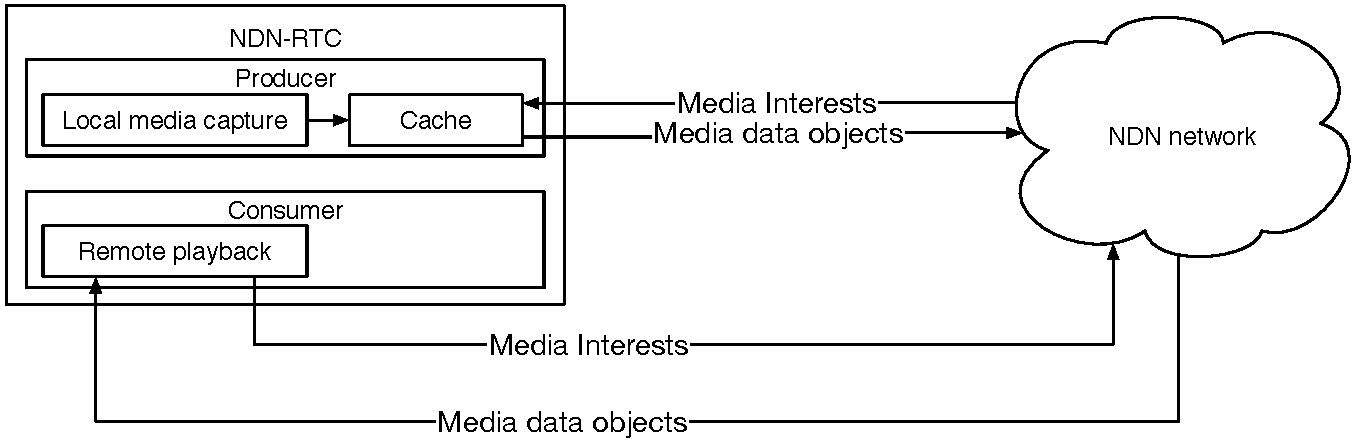
\includegraphics[width=0.5\textwidth]{architecture}
\caption{RTC over NDN}
\label{fig:arc}
\end{figure}

Figure \ref{fig:arc} presents top-level overview of how NDN-RTC works. Local media capture and Cache belong to the producer part of the NDN-RTC. Media is stored in the cache which provides access to the data for all incoming interests. Remote playback represents consumer: it issues interests, prepares received media (assembles video frames from segments and re-orders them) and plays it back.

\paragraph{Producer}

In case of video streaming, producer uses video encoding in order to reduce size of the frames. There are two types of encoded frames: \textit{Key} and \textit{Delta}. Key frames contain the most of the video information and don't depend on any previous frames to be decoded. Whereas Delta frames are dependent on all previous frames received after the last Key frame and can't be decoded without significant visual artifacts if any of those frames are missing.

Encoded frames vary in size, but average bitrate stays the same. For example, these are the average sizes of frames for 1000 kbps stream:
\begin{itemize}
\item \textbf{Key frames} $\approx$ 30KB;
\item \textbf{Delta frames} $\approx$ 3-7KB.
\end{itemize}

Therefore, depending on the underlying internet protocol used (IP in the existing NDN testbed), producer may need to segment encoded frames into a smaller chunks and provide clear naming conventions for consumer to fetch them (see Figure \ref{fig:producer}).

\begin{figure}[t!]
\centering
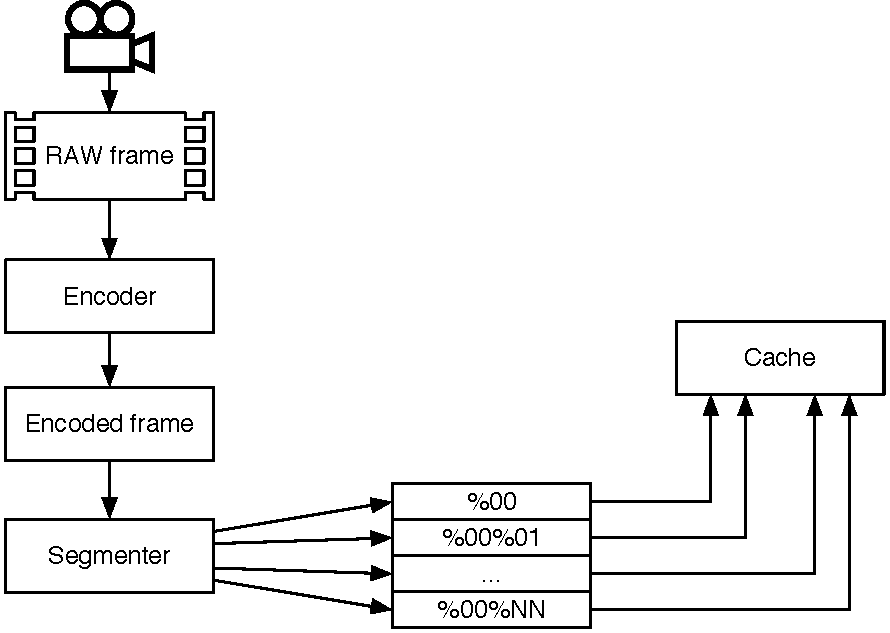
\includegraphics[width=0.5\textwidth]{producer}
\caption{NDN-RTC producer}
\label{fig:producer}
\end{figure}

\paragraph{Consumer}

Consumer takes into account that media packets are presented by separate segments in the network. Therefore, consumer implements mechanisms of interest pipelining and frame buffering (see Figure \ref{fig:consumer}). Interest pipeliner issues interests for individual segments and is controlled by some higher-level logic which achieves one out of four consumer's goals - ensures that only the latest data is fetched. Packets re-ordering, drops and latency fluctuations absorbtion are attained by the frame buffer which introduces buffering delay and re-arranges received frames in the playback order.

\begin{figure}[t!]
\centering
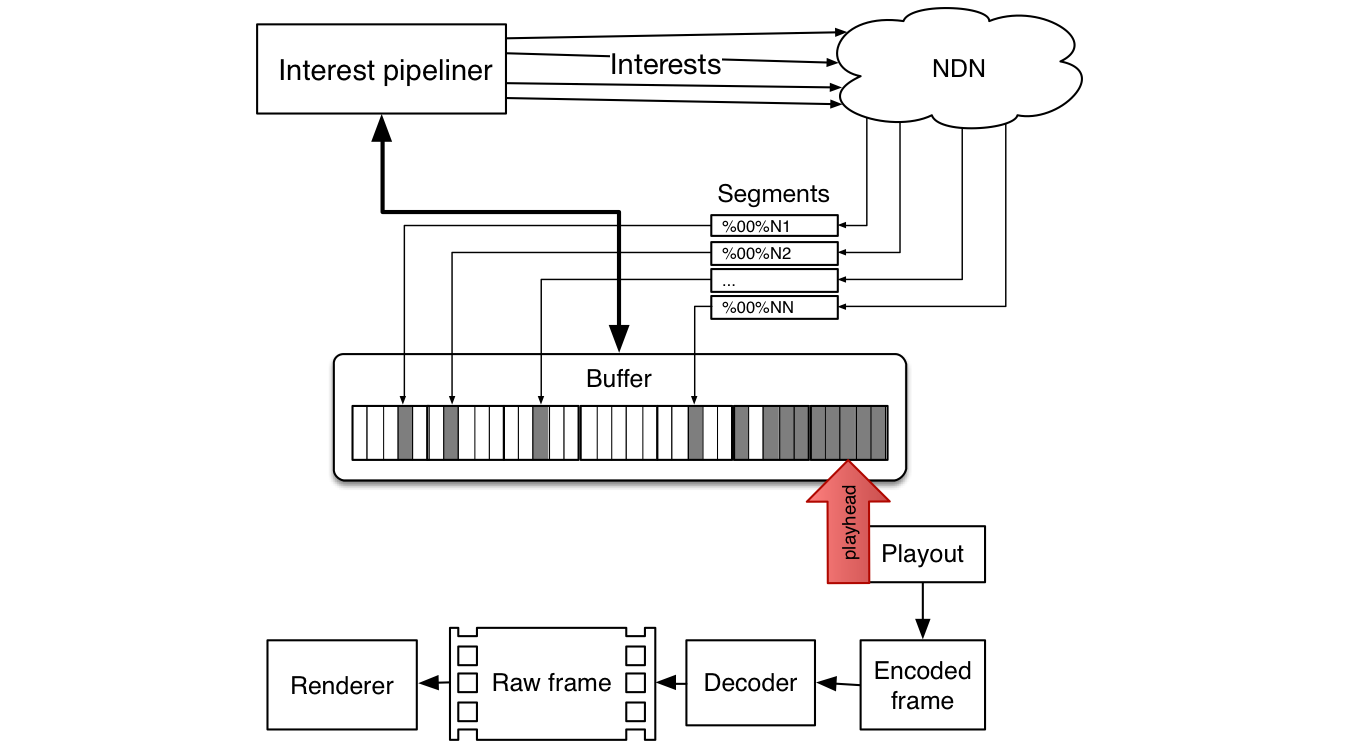
\includegraphics[width=0.5\textwidth]{consumer}
\caption{NDN-RTC consumer}
\label{fig:consumer}
\end{figure}


%************************************************
\subsection{Namespace}

As there is no direct consumer-produder communication, it is producer's job to provide as much supportive information as possible so that consumer is able to use this information in order to achieve her goals. There are several kinds of data producer can publish and these kinds should be reflected in the namespace:

\begin{itemize}
\item Media data
\begin{itemize}
\item Video frames
\item Audio samples
\end{itemize}
\item Forward error correction data
\item Producer's streams meta info
\end{itemize}

Besides that, the namespace should also reflect data specialization hierarchy - from general concepts in the root to more specialized entities towards the leaves. 

NDN-RTC producer uses a concept of \textit{media stream} for describing published media. Media stream represents a flow of raw media packets (video frames or audio samples) coming from an input device. Streams usually derive names from their input devices. It is quite natural for a producer to publish several media streams simultaneously, if she has more than one device to publish media from (for instance, publish video from camera, audio from microphone and another video stream for sharing computer screen). As all raw data should be encoded, the next level in the name hierarchy represents different encoder instances called \textit{media threads}. Thus, media threads allow producer to provide same media stream in several copies, for instance in low, medium and high quality for video, so that consumer can have a chance to choose media thread more suitable for the current network conditions.

\begin{figure}[t!]
\centering
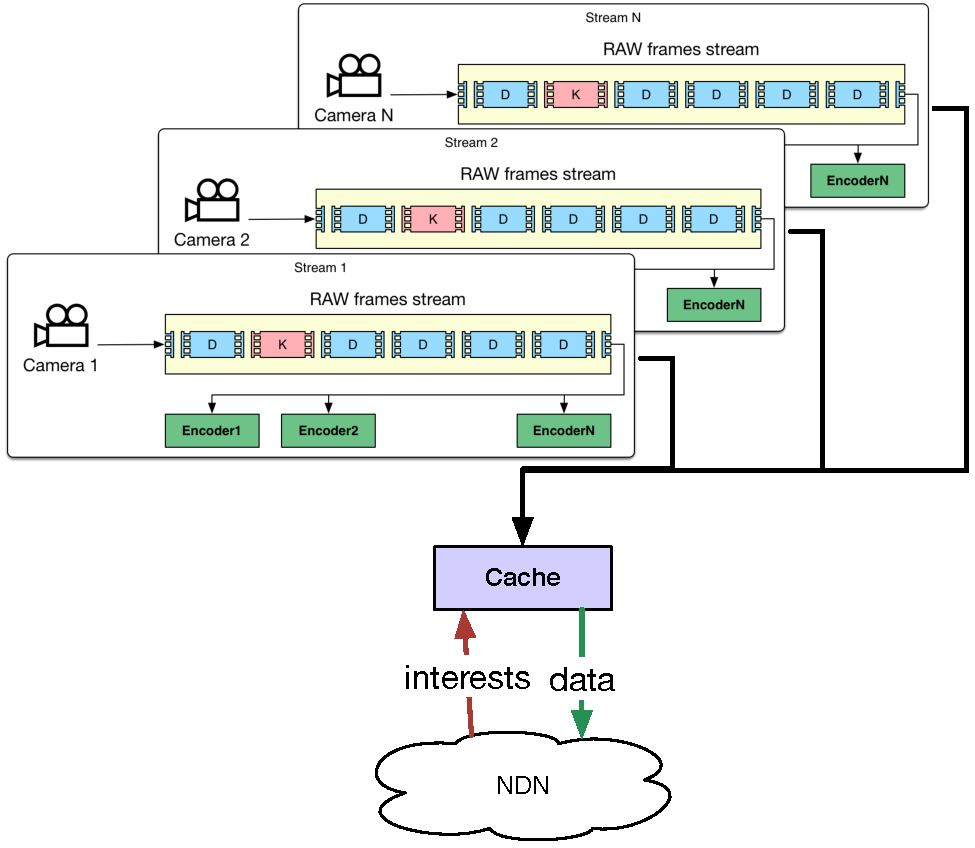
\includegraphics[width=0.5\textwidth]{streams-hierarchy}
\caption{NDN-RTC media streams hierarchy}
\label{fig:stream-hierarchy}
\end{figure}

NDN-RTC does not use any specific media container format for delivering its media to consumers. Instead, encoded media packets are segmented if needed and published under distinctive hierarchical names. Video frames are separated into two domains as per frame type: \textit{delta} and \textit{key} and numbered sequentially and independently. Both sequence numbers for delta and key frames start from 0. Next level specializes data type - it can be either media data or parity. Parity data, if producer opts to publish it, can be used by consumer to recover frames that miss one or more segments. The topmost level of the namespace defines individual data segments. These segments are also numbered suquentially and segment numbers conform to NDN naming conventions \cite{ndn_naming}.

There are some differences in case of the audio streams. First, there are no key frames, therefore all the audio packets are published under the \textit{delta} namespace. Second, audio samples are significantly smaller than video frames and do not require to be segmented. In practice, it appears that multiple audio samples can be bundled into one data segment. Therefore, instead of segmenting audio packets, they are bundled together until the size of one data segment is reached and published only after that.

Consumers need to know producer's streams structure in order to fetch data successfully. In order to save consumer from traversing actual producer's name tree, which can be time-consuming and unreliable, producer publishes meta information about her current streams under \textit{session info} component. Thus, consumers can retrieve up-to-date information about the producer's state.

\begin{figure}[t!]
\centering
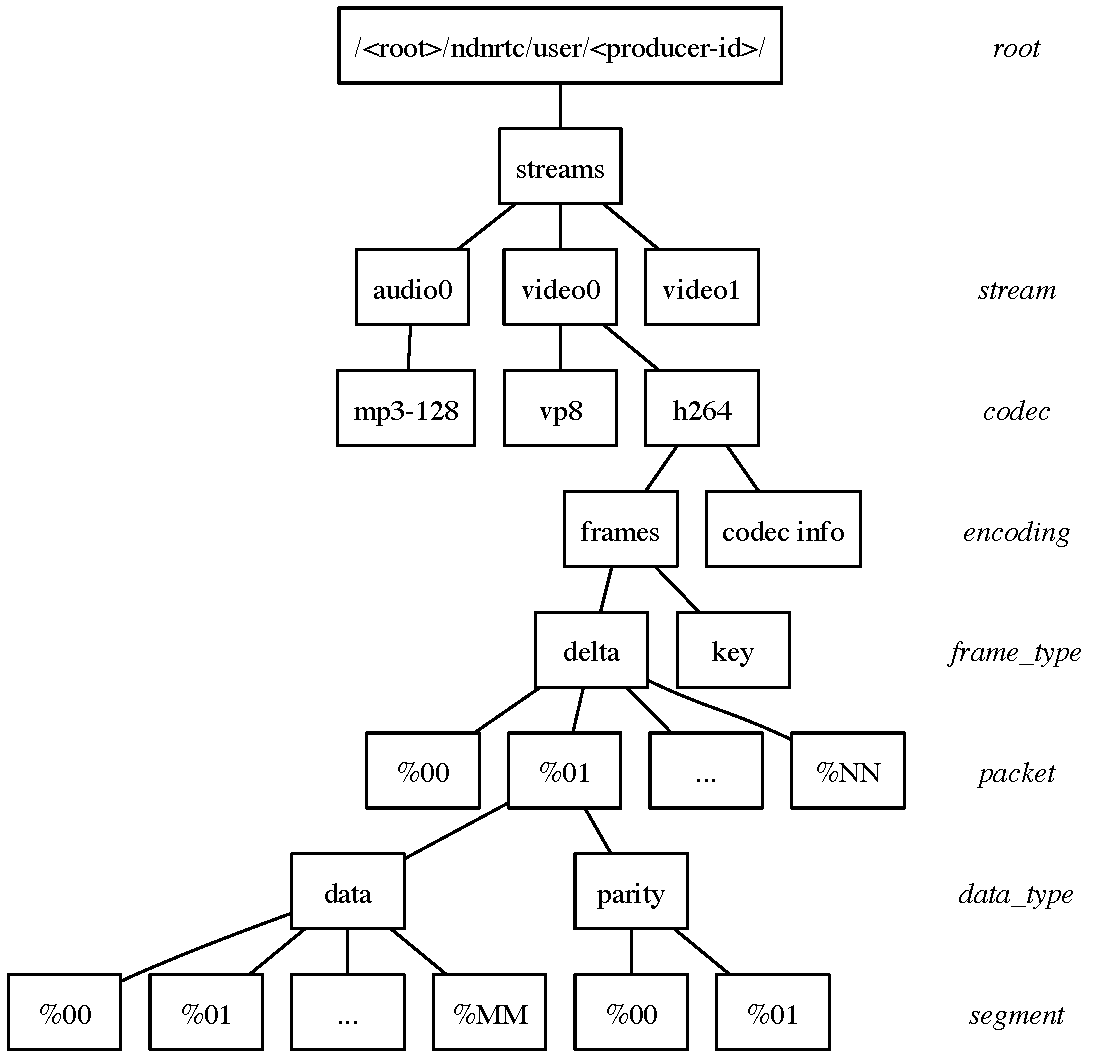
\includegraphics[width=0.5\textwidth]{namespace}
\caption{NDN-RTC namespace}
\label{fig:namespace}
\end{figure}

Besides naming data objects, data names can be appended by some additional media-level meta information which can be utlilized by consumers regardless of which frame segment was received first. Three components are added at the end of every data segment name:
\small\begin{equation}
.../\textbf{segment\#}/\textbf{playback\#}/\textbf{paired\_seq\#}/\textbf{num\_parity} \nonumber
\end{equation}\normalsize
\begin{itemize}
\item \textit{playback\#} - absolute playback number for current frame; this is different from the \textit{frame\#} which is a sequential number for the frame in its' domain (i.e. Key or Delta);
\item \textit{paired\_seq\#} - sequential number of the corresponding frame from other domain (i.e. for delta frames, it is sequential number of the corresponding key frame which is required for decoding);
\item \textit{num\_parity} - number of parity segments for this particular frame.
\end{itemize}


%************************************************
\subsection{Data objects}
Producer generates signed data objects from input media streams and places them in cache instantly. Incoming interests retrieve data from cache, if it is present, or forwarded further to the producer, if the requested data has not been produced yet. In such cases, producer maintains a pending interests table (PIT), which is checked every time new data object is generated. If an interest for newly generated data object exists in the PIT, it gets answered and PIT entry is erased.

\begin{figure}[t!]
\centering

\subfigure[video frame segmentation]{\label{fig:segment}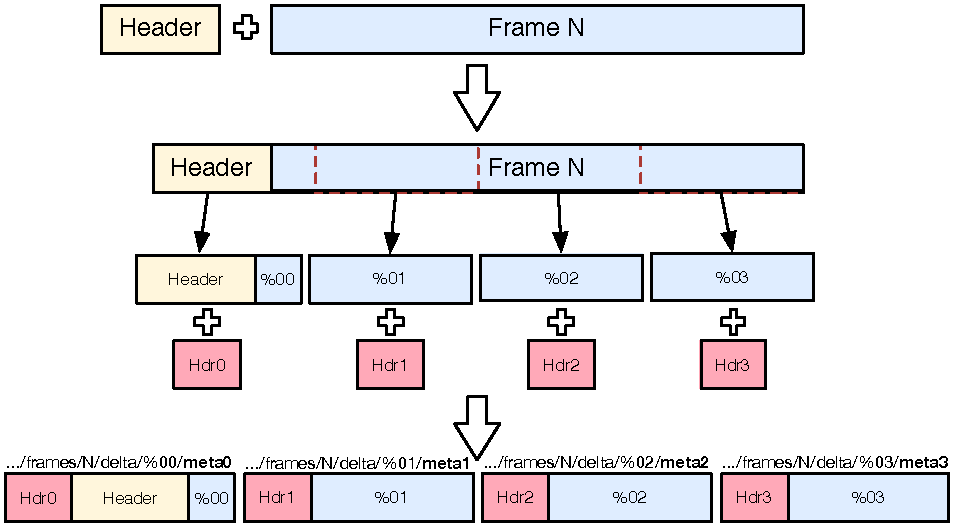
\includegraphics[width=0.5\textwidth]{segmentation}}
\subfigure[audio samples bundling]{\label{fig:audio-bundling}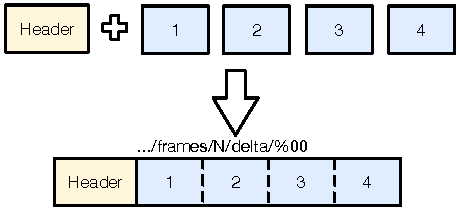
\includegraphics[width=0.3\textwidth]{audio-bundling}}

\caption{Segmentation and bundling}

\end{figure}

Besides actual stream data, data objects contain some amount of meta information which is prepended during frames segmenting (see Figure \ref{fig:segment}). There are two types of headers: \textit{Frame header} and \textit{Segment header}. Frame header is prepended to segment \#0 of each individual video frame and contains media-specific information (such as size of a frame), timestamp, current rate and unix timestamp, which can be used for calculating actual delay between NTP-synchronized producer and consumers (see Figure \ref{fig:data-struct}). Segment header is prepended to every segment of a frame. It carries network-level information which can be used by consumer for making certain assumptions about current network conditions and origin of the data objects received:
\begin{itemize}
\item Interest nonce

Nonce value of the interest which requested this particular segment. There are three meaningful cases: 
\begin{itemize}
\item \textit{value belongs to the interest issued previously} - consumer received non-cached data requested by interest issued previously;
\item \textit{value is non-zero, but doesn't belong to any of the previously issued interests} - consumer received data requested by some other consumer; data may be cached;
\item \textit{value is zero} - consumer received data which was cached on producer side and never requested by anyone before.
\end{itemize}

\item Interest arrival timestamp

Timestamp of the interest arrival. Monitoring this value and interest expression timestamps over time may give consumer a clue about how long does it take for interests to reach producer. This value is only valid when nonce value belongs to one of the consumer's interests.

\item Generation delay

Time interval in milliseconds between interest arrival and segment publishing. Consumer can use this value to her advantage in order to control the number of outstanding interests. This value is only valid when nonce value belongs to one of the consumer's interests.

\end{itemize}

\begin{figure}[t!]
\centering
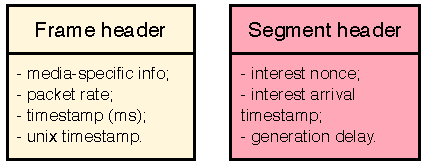
\includegraphics[width=0.3\textwidth]{data-struct}
\caption{Frame and segment headers}
\label{fig:data-struct}
\end{figure}

Audio samples are not prepended by any segment header, however the whole audio bundle is prepended by the same frame header (see Figure \ref{fig:audio-bundling}).

%************************************************
\subsection{Consumer protocol}

%************************************************
\subsubsection{Frame fetching}

Consumer doesn't know the total number of segments beforehand, unless the very first segment is fetched - in this case, consumer can retrieve metadata from the received segment and get total number of segments for the current frame. 
Therefore, at first attempt, consumer tries to make a "best guess" in the number of segments she needs to fetch by issuing $M$ interests (see Figure \ref{fig:pull}). If interests arrive too early, they will be added to the producer's PIT and stay there for some amount of time $d_{gen}$ called \texttt{generation delay}. Once encoded frame is segmented into $N$ segments, they are published and if $N\geq M$, interests $0 - M$ are answered with the data  which travels back to consumer. Upon receiving first data segment, consumer determines the total number of segments for the current frame and issues $N - M$ more interests for the missing segments if any. These segments will be satisfied by data with no generation delay (as the frame has been published already by producer). The time interval between receiving very first segment and until the frame is fully assembled is represented by $d_{asm}$ and called \texttt{assembling time}.

\begin{figure}[t!]
\centering
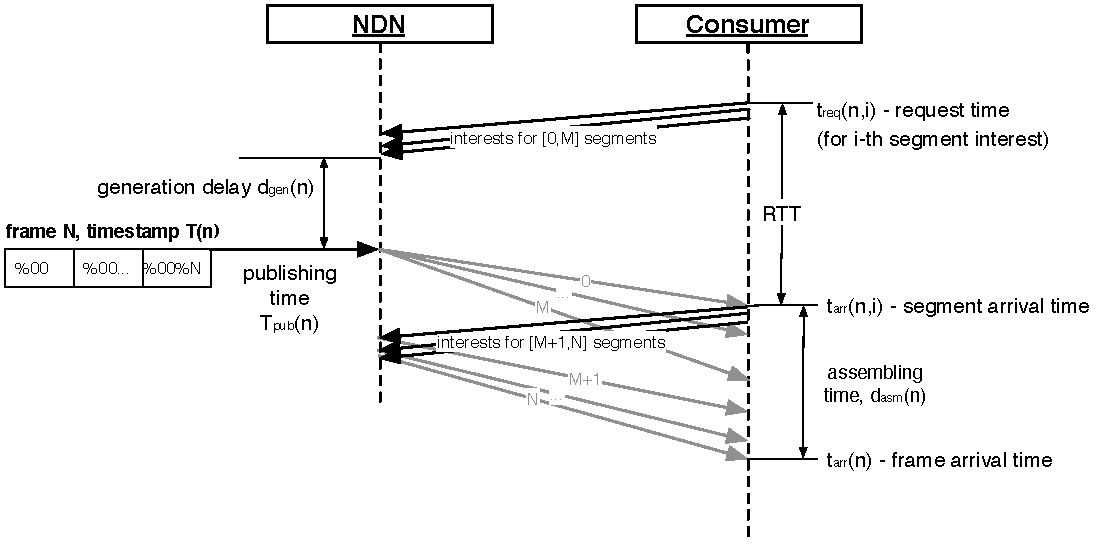
\includegraphics[width=0.5\textwidth]{frame-fetch}
\caption{Fetching frame}
\label{fig:pull}
\end{figure}

It is needlesss to say, that additional round-trips for requesting missing data segments increase overall frame assembling time and chances that the frame will be incomplete by the time it should be played back. This problem could have been avoided if consumer could make a better guesses in the number of initial interests. Therefore, the following considerations were introduced in later versions of the library:
\begin{itemize}
\item consumer should know what type of frame she is going to fetch (as average number of segments varies greatly for different frame types);
\item consumer should track average number of segments per frame type.
\end{itemize}

The first consideration was implemented by introducing separate namespaces for key and delta frames. The second consideration helps consumer do better at guessing the number of initial interests.

\subsubsection{Bufferization}

% Buffer:
% - re-ordering
% - added latency to mitigate network delays
% - extended defition:
% 	- pending frames
% 	- assembling frames
% - buffer-based retransmissions

As in traditional streaming applications, consumer uses frame bufferization in order to tackle out-of-order data arrivals and network delay deviations. Consumer-side jitter buffer is also used as a place for assembling frames by segments. However, the definition of jitter buffer is extended for NDN networks. In traditional push-based approach, buffer can not contain empty frame slots - they are allocated/reserved only when data arrives. Pull-based paradigm requires consumer to request data explicitly. Therefore, after expressing interest consumer "knows" that new data is coming and a frame slot should be reserved in the buffer. Practically, this means, that there will always be some number of empty reserved slots in the buffer. Thus, jitter buffer's size have two measurements:
\begin{itemize} 
\item \textit{playback size} - playback duration of all complete ordered frames by the moment;
\item \textit{estimated size} = \textit{playback size} + \textit{number of reserved slots} $\times$ 1/\textit{producer rate}
\end{itemize}

The difference between estimated size and playback size ($RTT^{\prime}$) can't be smaller than the current average RTT value. In fact, keeping this value at a minimum indicates that consumer receives the most recent data with the minimal amount of outstanding interests. Monitoring this value over time may help consumer to get a clue on her "sync" status with the producer. For example, consumer may use it during fetching process as will be discussed in the next section. 

\subsubsection{Fetching process}

For RTC applications it is critical to receive the most recent data from the network as well as to preserve it's caching ability for proper scaling. Consumer should not merely rely on using such flags as \textit{AnswerOriginKind} and \textit{RightMostChild}. The high frequency nature of streaming data makes no guarantees that the data satisfying those flags received by a consumer will be the most recent one. Instead, consumer should use other indicators to ensure that the network supplies up-to-date stream data. The fact that the media data is published with constant rate means that inter-arrival delays ($D_{arr}$) of the most recent samples repeat this publishing pattern. In contrast, cached data will follow interest expression pattern. Therefore, by monitoring inter-arrival delays of consequtive media samples, consumer can make assumptions about data freshness (see Figure \ref{fig:inter-arrival}).

\begin{figure}[t!]
\centering

\subfigure[bursty cached data arrival, reflects interests expression pattern]{\label{fig:cached}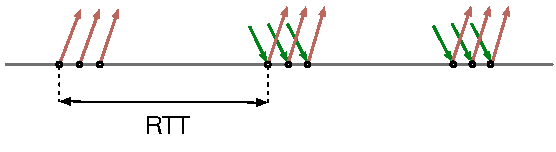
\includegraphics[width=0.4\textwidth]{arrival-cached}}\\
\subfigure[stable fresh data arrival, reflects publishing pattern]{\label{fig:fresh}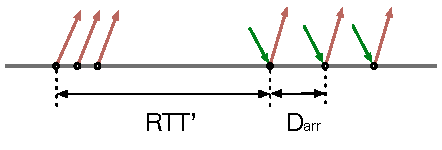
\includegraphics[width=0.35\textwidth]{arrival-fresh}}

\caption{Arrival patterns for the cached and most recent data}
\label{fig:inter-arrival}
\end{figure}

During bootstrapping, consumer "chases" producer and aims to exhasut network cache. By incerasing the number of outstanding interests, consumer "pulls cached data" out of the network unless the freshest data starts to arrive. After that, the number of outstanding interests may be decreased. 

In order to control interest expresssion, a concept of $W$ is introduced (see Figure \ref{fig:w-concept}). Consumer expresses interests only when $W > 0$. At every moment, $W$ indicates how many outstanding interests can be sent out. Before the bootstrapping phase, consumer initializes $W$ with some value. This value should reflect consumer's idea on how many interests are needed in order to exhaust network cache and reach the most recent data (Figure \ref{fig:ws} shows how bigger value of $W$ helps to exhaust cache faster). Every time a new interest is expressed, $W$ gets decremented. When new data arrives, $W$ is incremented, thus allowing consumer to issue more interests. Hence, even though interest expression is data-driven, number of outstanding interests is controlled by a consumer and directly influences how fast consumer can "chase" producer.

\begin{figure}[t!]
\centering

\subfigure[$W$ concept]{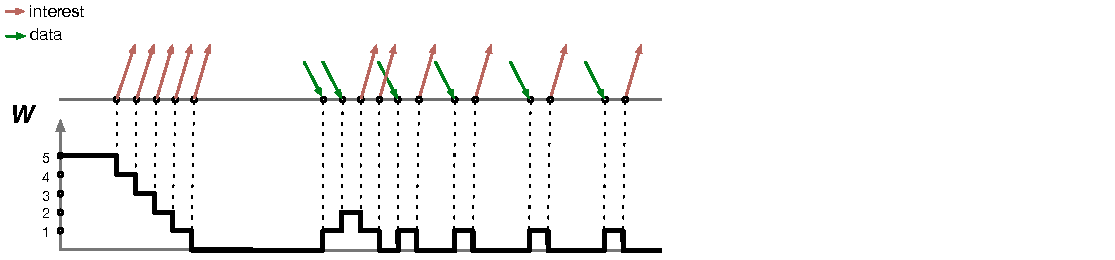
\includegraphics[width=0.35\textwidth]{w-concept}}
\subfigure[interests bursting ($W+3$)]{\label{fig:int-burst}
\includegraphics[width=0.35\textwidth]{int-burst}}
\subfigure[interests withholding ($W-3$)]{\label{fig:int-hold}
\includegraphics[width=0.35\textwidth]{int-hold}}

\caption{Interest expression control}
\label{fig:w-concept}
\end{figure}

\begin{figure}[t!]
\centering
%\captionsetup[subfigure]{aboveskip=-1pt,belowskip=-2pt}
\begin{scriptsize}
\subfigure[$W=10$: short chasing, bigger $RTT^\prime$]{\def\svgwidth{0.48\textwidth}\input{w10.pdf_tex}}
\subfigure[$W=4$: longer chasing, smaller $RTT^\prime$]{\def\svgwidth{0.48\textwidth}\input{w4.pdf_tex}}
\subfigure[$W=3$: consumer can't exhasut cache, $RTT^\prime = RTT$]{\def\svgwidth{0.48\textwidth}\input{w3.pdf_tex}}
\end{scriptsize}
\caption{Bigger $W$ decreases "chasing" phase, but increases $RTT^\prime$ for the same network configuration ($RTT\approx100ms$)}
\label{fig:ws}
\end{figure}

$W$ provides a simple mechanism which can be used to speed up or slow down interests expression. Any increase in $W$ value makes consumer to issue more interests (Figure \ref{fig:int-burst}), whereas decrease in $W$ holds consumer back from sending any new interests (Figure \ref{fig:int-hold}). Bigger values of $W$ makes consumer faster reach synchronized state with producer. However, larger value means larger number of outstanding interests and bigger $RTT^\prime$ because of longer generation delays $d_{gen}$ for each media sample. By adjusting the value of $W$ and observing inter-arrival delays $D_{arr}$ consumer can find minimal $RTT^\prime$ value while still getting non-cached data, thus achieving best synchronization state with producer.

For more complex scenario of video streaming, consumer controls expression of "bulks" of interests instead of individual interests, because video frames are composed of several segments. In this case, $W$ is adjusted on per-frame basis, rather than per-segment. In all other respects, the same above logic can be applied.

Bootstrapping phase starts with issuing interest with enabled \textit{RightMostChild} selector in delta namespace for audio and key namespace for video. The reason, why this process differs for video streams is that consumer is not interested in fetching delta frames without having corresponding key frame for decoding. Once initial data segment of sample with number $S_{seed}$ has been received, consumer initializes $W$ with some initial value $N$ and asks for the next sample data $S_{seed}+1$ in the appropriate namespace. Upon receiveing first segments of sample $S_{seed}+1$, consumer initiates fetching process described above for all namespaces (delta and key, if available). Bootstrapping phase stops when consumer finds minimal value of $W$ which still allows receiving the most recent data - i.e. consumer reaches synchronized state with producer and switches to a normal fetching phase where no adjustments for $W$ are needed. 
% Listing \ref{lst:fetch-algo} shows pseudo-code for the bootstrapping phase.

% \begin{algorithm}
% \begin{algorithmic}

% \Function{Bootstrap}{Meta}

% \If {audio}
% 	\State $Nspc \gets DeltaNamespace$
% \Else
% 	\State $Nspc \gets KeyNamespace$
% \EndIf

% \State \Call{ExpressOne}{$RightMostChild$, $Nspc$}
% \Ensure Received data segment $Dseed$
% \State $Sseed \gets$\Call{GetSeqNumber}{$Dseed$}
% \State $NavgKey \gets$\Call{GetAvgSegNum}{$Meta$, $Key$}
% \State \Call{ExpressBulk}{$NavgKey$, $Sseed+1$, $Nspc$}
% \Ensure Received data segment $D$ for $Sseed+1$
% \State $J \gets$ \Call{GetDeltaNumber}{$D$}
% \State $NavgDelta \gets$\Call{GetAvgSegNum}{$Meta$, $Delta$}
% \State $DW \gets N$
% \State $W \gets DW$

% \While{$BootstrappingPhase$}

% \While{$W > 0$}
% 	\State \Call{ExpressBulk}{$NavgDelta$, $J$, $Delta$}
% 	\State $W \gets W-1$
% 	\State $J \gets J+1$
% \EndWhile

% \If {received segment $Dj$ for new sample}
% 	\State $W \gets W+1$
% \EndIf

% \EndWhile

% \State \Call{Switch}{$FetchingPhase$}

% \EndFunction

% \end{algorithmic}

% \label{lst:fetch-algo}
% \caption{Bootstrap}
% \end{algorithm}

\section{Implementation}
TBD

\section{Evaluation}
TBD

\section{Issues and future work}
TBD

\section{Conclusion}

\end{document}